% Preamble
\documentclass[a4paper,12pt]{article}

\usepackage[osf]{mathpazo} % palatino
\usepackage{ms}            % load the template
\usepackage[round]{natbib} % author-year citations
\usepackage{graphicx}
\usepackage{parskip}      
\pagenumbering{arabic}    
\linespread{1.66}

% Title page information
\title{Shedding Light on the ``Dark Side'' of Phylogenetic Comparative Methods}
\author{
  Natalie Cooper$^{1,2,*}$, Gavin H. Thomas$^{3}$\\ and Richard G. FitzJohn$^{4}$
}
\date{}
\affiliation{\noindent{\footnotesize
  $^1$ School of Natural Sciences, Trinity College Dublin, Dublin 2, Ireland.\\ 
  $^2$ Department of Life Sciences, Natural History Museum, Cromwell Road, London, SW7 5BD, UK.\\
  $^3$ Department of Animal and Plant Sciences, University of Sheffield, Sheffield, S10 2TN, UK.\\
  $^4$ Department of Biological Sciences, Macquarie University, Sydney, NSW 2109, Australia. \\
  $^*$ Corresponding author: natalie.cooper@nhm.ac.uk; Department of Life Sciences, Natural History Museum, Cromwell Road, London, SW7 5BD, UK. Fax: +353 1 677 8094; Tel: +353 1 896 5083.\\
}}

\vfill

\runninghead{The dark side of phylogenetic comparative methods}
\keywords{PCM, assumption, bias, caveat, phylogenetic independent contrasts, Ornstein-Uhlenbeck, trait-dependent diversification\\
\textbf{Word count}: 3508 (including references, tables and figure legends)}

% End of preamble

\begin{document}
\modulolinenumbers[1]   % Line numbering on every line

\mstitlepage

\parindent = 1.5em
\addtolength{\parskip}{.3em}

% Abstract 350 words max
\section{Abstract}

Phylogenetic comparative methods are becoming increasingly popular for investigating evolutionary patterns and processes.
However, these methods are not infallible - they suffer from biases and make assumptions like all other statistical methods.
Unfortunately, although these limitations are often well-known in the phylogenetic comparative methods community, they are often inadequately assessed in empirical studies leading to misinterpreted results and poor model fits.
Here we explore reasons for the communication gap dividing those developing new methods and those using them. 
We suggest that some important pieces of information are missing from the literature, and that others are difficult to extract from long, technical papers.
We also highlight problems with users jumping straight into software implementations of methods (e.g. in R) that may lack documentation of biases and assumptions that are mentioned in the original papers.
To help solve these problems we make a number of suggestions including providing
blog posts or videos to explain new methods in less technical terms, encouraging reproducibility and code sharing, wiki-style pages summarising the literature on popular methods, more careful consideration and testing of whether a method is appropriate for a given question/dataset, incentives for collaboration, and a shift from publishing purely novel methods to publishing improvements to existing methods, and ways of detecting biases or testing model fit.
Many of these points are applicable across methods in ecology and evolution, not just phylogenetic comparative methods.

\newpage
\raggedright
\doublespacing
\setlength{\parindent}{1cm}

%----------------------------
\section{Introduction} 

A long time ago in a galaxy far, far away - also known as the 1980s - phylogenetic comparative methods (PCMs) were first developed. 
These methods use information on the evolutionary relationships of organisms to compare species \citep{harvey1991comparative}, and were initially designed to deal with the statistical non-independence of species in comparative analyses (e.g. \citealp{felsenstein1985phylogenies,grafen1989phylogenetic}).  
Since then PCMs have been extended to investigate evolutionary pattern and process (see reviews in \citealp{o2012evolutionary, pennell2013integrative}), and include methods for investigating drivers of diversification \citep[e.g.][]{maddison2007estimating}, the tempo and mode of trait evolution \citep[e.g.][]{o2012evolutionary}, and models of speciation and extinction \citep[e.g.][]{nee1994extinction}. 
PCMs have also become extremely popular over recent years; the number of papers containing the phrase ``phylogenetic comparative'' has increased dramatically since the 1980s (Figure \ref{PCMCitations}). 
With new methods being published almost weekly, there has never been a better time to be a comparative biologist.

Unfortunately, PCMs also have a ``dark side''; they make various assumptions and suffer from biases in exactly the same way as any other statistical method - a fact that is well established in the literature \citep[e.g.][]{freckleton2009seven,losos2011seeing,blomberg2012independent,boettiger2012your}.
Increasingly however, assumptions and biases are inadequately assessed in empirical studies, leading to poor model fits and misinterpreted results (see examples below).
Additionally, little consideration is given to whether using a PCM is really appropriate for the question at hand \citep{westoby1995misinterpreting,losos2011seeing}. 

We suggest that one cause of this problem is that although researchers developing and implementing new methods are aware of the limitations of their methods and the assumptions that underly them, this information is not always being effectively transferred to end-users.
Additionally, the tools and approaches used to fit models are often far more user-friendly and better documented than the methods used to to assess whether that model fit is reasonable. 
Clearly more effort is needed to bridge the widening gap between those developing methods and end-users. 
Here we explore the causes of this communication gap and suggest some potential solutions.
Note that many of these issues are applicable across methods in ecology and evolution, not just PCMs.

\subsection{Examples of the problem}
Before exploring the reasons behind the communication gap, we give three brief examples of commonly used PCMs that have assumptions, biases or caveats that are often inadequately assessed in empirical studies.
Because the aim of this paper is to provide positive ways to move forward, rather than to admonish authors for past errors, we do not cite papers we feel have fallen into these traps (especially as we are guilty of making some of the same mistakes). 

\subsubsection{Phylogenetic independent contrasts}
The phylogenetic independent contrasts method uses phylogenetic information to account for the fact that species in a comparative analysis are related to each other and thus may share similarities because they inherit them from their ancestors, not because of independent evolution \citep{felsenstein1985phylogenies,harvey1991comparative}. 
This is the most commonly used phylogenetic comparative method (\citet{felsenstein1985phylogenies} has been cited nearly 6000 times; Google Scholar search 10th October 2015), and a great deal of literature exists on the assumptions underlying the method, and ways of testing whether these assumptions are met. 
The method has three major assumptions (although there are many more than this) \citep{diaz1996testing}, (1) that the topology of the phylogeny is accurate; (2) that the branch lengths of the phylogeny are correct; and (3) that traits evolve in the manner of the Brownian constant variance model, a simple model of trait evolution where trait variance accrues as a linear function of time \citep{cavalli1967,felsenstein1973maximum}.
The third assumption is stated in \citet{felsenstein1985phylogenies} though the other two are not explicitly mentioned. 
However each assumption is explored in many subsequent papers \citep[e.g.][]{felsenstein1988phylogenies,grafen1989phylogenetic,harvey1991comparative,garland1992procedures,purvis1995comparative,diaz1996testing,hansen1996translating,martins1997phylogenies,freckleton2000phylogenetic,garland2000using,hansen2005assessing,freckleton2006detecting,rohle2006comment}.
There are several ways of testing these assumptions, including looking for relationships among standardised contrasts and node heights \citep{grafen1989phylogenetic,freckleton2006detecting}, absolute values of standardised contrasts and their standard deviations \citep{garland1992procedures,diaz1996testing}, and heteroscedasticity in model residuals \citep{purvis1995mammal}.
These tests are fairly easy to implement and are included as standard model diagnostic plots in CAIC and the \texttt{caper} R package \citep{purvis1995comparative,Orme:2013aa,R-Core-Team:2014aa}.
However, the majority of studies using phylogenetic independent contrasts do not mention testing these assumptions (\citealp{freckleton2006detecting}; although they may have tested the assumptions and not recorded this).
In addition, because phylogenetic independent contrasts are identical to phylogenetic generalised least squares models \citep{garland2000using,rohle2006comment,blomberg2012independent}, these models also have the same assumptions that are equally rarely addressed. 

\subsubsection{Ornstein-Uhlenbeck models of trait evolution}
Most models of trait evolution are based on the Brownian constant variance model \citep{cavalli1967,felsenstein1973maximum}.
The Ornstein-Uhlenbeck (OU) model is a modification of the Brownian model with an additional parameter that measures the strength of return towards a theoretical optimum shared across a clade or subset of species \citep{hansen1997stabilizing,Butler:2004aa}.
OU models have become increasingly popular as they tend to fit the data better than Brownian motion models, and have attractive biological interpretations \citep{cooper2016}.
For example, fit to an OU model has been seen as evidence of evolutionary constraints, stabilising selection, niche conservatism, and selective regimes \citep{Wiens:2010aa,beaulieu2012modeling,christin2013anatomical,mahler2013exceptional}.
However, the OU model has several well-known caveats \citep[see][]{ives2010phylogenetic,boettiger2012your,hansen2012interpreting,ho2013asymptotic,ho2014intrinsic}. 
For example, it is frequently incorrectly favoured over simpler models when using Likelihood ratio tests, particularly for small datasets that are commonly used in these analyses (the median number of taxa used for OU studies is 58; \citealp{cooper2016}). 
Additionally, very small amounts of error in datasets can result in an OU model being favoured over Brownian motion simply because OU can accommodate more variance towards the tips of the phylogeny, rather than due to any interesting biological process \citep{boettiger2012your,pennell2015model}.
Finally, the literature describing the OU model is clear that a simple explanation of clade-wide stabilising selection is unlikely to account for data fitting an OU model \citep[e.g.][]{hansen1997stabilizing,hansen2005assessing}, but users of the model often state that this is the case.
Unfortunately, these limitations are rarely taken into account in empirical studies.

\subsubsection{3. Trait-dependent diversification} % Gavin - I could do with your help here, not so sure on these methods but it seemed like a timely example.
Analyses of trait-dependent diversification are used to detect whether particular traits promote high rates of diversification, leading to some clades becoming more diverse than others \citep{nee1994reconstructed}. 
These kinds of analyses have been applied extensively in recent years to a variety of taxa and traits \citep[e.g.][]{}. % add citations
Most use the binary-state speciation and extinction model (BiSSE) and related methods (the original BiSEE paper \citet{maddison2007estimating} has been cited 384 times; Google Scholar search 10th October 2015).
However, \citet{rabosky2015model} recently reevaluated the method and its assumptions and showed via simulations that a strong correlation between a trait and diversification rate can be inferred from a single diversification rate shift within a tree, even if the shift is unrelated to the trait of interest.
They suggest that many examples of trait-dependent diversification actually reflect this rate heterogeneity in trees, and thus are biologically meaningless.
Interestingly, these caveats are mentioned in earlier papers \citep{maddison2007estimating,fitzjohn2010quantitative,FitzJohn:2012aa} but were seemingly not widely understood given the shock reaction to \citet{rabosky2015model}.

\subsection{What impedes information transfer about the limitations of PCMs?}
These three brief examples illustrate that although the PCM community is aware of the limitations of PCMs, this information is not filtering through to everyone using the methods. 
Why might this be the case?

  \subsubsection{1. Not everything is mentioned in the literature}
    As scientists we mainly communicate our ideas through the literature. 
    Unfortunately, some of the information needed to properly apply PCMs is not found in the literature. 
    We refer to this knowledge as ``PCM folklore'' because it tends to be passed down from PIs to graduate students (and it is occasionally closer to fiction than fact!).
    Sometimes the folklore includes tricks to get methods working, or useful rules-of-thumb; other times it is more opinion-based, but over time these opinions become rules. 
    Useful PCM folklore is often shared among developers, and among collaborating groups, but is not always shared outside of these circles. 
    When it is shared, it tends to be as email exchanges of ``dark advice'' that is not accessible to the rest of the community.

    One example of PCM folklore is that species with Studentized residuals $\pm 3$ are often omitted from regressions of phylogenetic independent contrasts, to avoid highly influential outliers affecting the results \citep[e.g.][]{GEB:GEB355}. 
    The rationale for this comes from \citet{jones1997optimum}, however, the $\pm 3$ cut-off is arbitrary, and barely mentioned in the original paper, but has become a rule-of-thumb for running these analyses (the paper has been cited \textgreater 100 times, mostly as a justification of this procedure).
    Another example is in the defaults of programs that perform PCMs. 
    These often start out as arbitrary starting points for data exploration with no justification for their use, but over time become the way the analysis is always performed.
    For example, % Anyone got a good example here?

    Other information about the limitations of a method may be absent from the literature due to the time-lag between a new method being published and others having time to test it. 
    For example, Felsenstein published the phylogenetic independent contrasts method in 1985 \citep{felsenstein1985phylogenies}, but it was not until the early 1990s that thorough critiques of the method and its assumptions began to be published \citep[e.g.][]{garland1992procedures}.
    This time-lag is shorter with more recent methods because simulations testing the method are now required by journals (although simulations only show that the method behaves appropriately under ideal conditions).
    However, we suspect there are still many hidden assumptions and biases in all PCMs, even established methods, that have yet to be properly explored in the literature.
    For example, see Maddison \& FitzJohn's (\citeyear{maddison2014unsolved}) recent critique of Pagel's (\citeyear{pagel1994detecting}) correlated evolution method, and Rabosky \& Goldberg's (\citeyear{rabosky2015model}) discussion of trait-dependent speciation models \citep{nee1994reconstructed,maddison2007estimating}.

  \subsection{2. The literature is too technical and/or important details are difficult to locate}
    Although some information is not found in the literature (see above), the majority of assumptions and biases of PCMs are documented somewhere. 
    A big issue for novice methods-users (and often for advanced users too) is that this information can be extremely technical and dense.
    It is not unusual for papers to be full of equations, \textgreater 20 pages long, and written in a way that gives one a headache. 
    Additionally there is a lot of literature to wade through before getting all of the required information. 
    For example, one of us (NC) recently reviewed papers discussing the assumptions and limitations of phylogenetic independent contrasts \citep{felsenstein1985phylogenies}, including how they are related to phylogenetic generalised least squares models \citep{garland2000using,rohle2006comment,blomberg2012independent}. 
    Even with prior knowledge of the key papers and authors to focus on, this resulted in $\approx 300$ manuscript pages and a book to read.
    This seems like an excessive amount of reading to run a simple empirical analysis.
    Another issue is that it can sometimes be hard to find the information required. 
    Assumptions and caveats can be found in the Introduction, Methods, Results and/or Discussion of a paper. 
    They are rarely neatly corralled in one place, making it easy to miss pertinent details. 

  \subsection{3. Users jump straight to the implementation of the method}
    In the early days of PCMs, some researchers provided stand alone packages to run their methods (e.g. PDAP; \citealp{diaz1996testing}), others provided code in whichever language they chose to program in (e.g. MATLAB code; \citealp{rohlf2001comparative}), and still others provided no way of implementing their methods at all. 
    This resulted in many frustrating hours (and days and months) trying to implement any new method you wanted to use.\\

    More recently however, the community has moved towards mostly implementing methods in R (\citealp{R-Core-Team:2014aa}; for a list of packages see Brian O'Meara's ``CRAN Task View: Phylogenetics, Especially Comparative Methods'' http://ftp.iitm.ac.in/cran/web/views/Phylogenetics.html), and code sharing has become almost ubiquitous. 
    The number of R packages for PCMs has increased sharply since 2005 when APE \citep{Paradis:2004aa} was released, and has increased particularly sharply since 2008 (Figure \ref{PCMRpackages}).
    Simultaneously, more people are able to use R thanks to workshops and changes in student training, thus when a new method is published it is now possible to take an R package ``off the shelf'' and use it to run the method immediately.
    \citet{freckleton2009seven} suggested that the ability to to conduct PCMs in flexible computing environments such as R would improve our ability to implement methods correctly. 
    However, this has instead led to an increasing number of people (including the authors) jumping straight to the implementation of a method, without fully understanding what the method is doing, what its assumptions might be, or what the results mean in a biological context.
    This problem is exacerbated by the fact that manuals, vignettes and help files for R packages rarely mention the assumptions of the method, or how to test model fit. 
    The APE book \citep{paradis2011analysis} for example, provides no guidance on assumption testing in its chapter on phylogenetic independent contrasts, even though the methods needed to do this are well-established and very easily implemented in R (for a counter example see CAIC and caper documentation; \citealp{purvis1995comparative,Orme:2013aa}).

\subsection{How can we solve some of these problems?}
  \subsubsection{1. Simplify, summarize and share}
    Many of the problems above are caused by methods papers being difficult to read. 
    This is not entirely the fault of those writing these papers; most journals have strict word limits so it is often easier to use a one line equation rather than a paragraph of description. 
    However, it is hard to complain about novice users failing to understand a method when the paper is incomprehensible.
    One solution is to prepare an accompanying blog post or video explaining the method in less technical terms. 
    Some journals already encourage this (including the British Ecological Society journals; see https://soundcloud.com/besjournals, https://www.youtube.com/user/MethodsEcolEvol), and even if they do not, there is no harm in doing this and hosting it on a personal website. 
    The ability to share ideas with a non-technical audience is a key skill to develop, and may encourage more people to use the method.
    Encouraging increased efforts at reproducibility would also help, by including knitR \citep{Xie:2015aa} reports in Supplementary Material showing exactly how each analysis was run \citep[e.g.][]{fitzjohn2014much}, or by requiring all analyses and code to be available on GitHub or Bitbucket. 
    At the very least, having a list of the main assumptions, biases and caveats of the method somewhere obvious would reduce misuse and provide a place to point people to when they begin using a method (this will be difficult as there are often hidden assumptions in a method, and listing all possible assumptions and caveats may be unfeasible in some cases).

    The glut of literature that already exists for established methods is a bigger problem.
    The Oxford Bibliographies Evolutionary biology pages have lists of key papers (http://www.oxfordbibliographies.com/obo/page/evolutionary-biology), but these are curated by just a few individuals and tend to contain a lot of papers. 
    One solution would be to establish a wiki-style website where people could post summaries of commonly used methods, along with lists of key papers to read. 
    The community would be responsible for peer reviewing these summaries to ensure all opinions are covered. 
    Erick Matsen's Phylobabble discourse page (http://phylobabble.org/) is an excellent example of a similar approach for phylogenetics. 
    The British Ecological Society's Quantitative Ecology Special Interest Group is also in the process of creating a ``Field Guide for Ecologists'' (http://bes-qsig.github.io/fge/) that will fill a similar niche in ecological methods.
    Unfortunately there is currently little incentive for people to contribute to such a project at the cost of time pursuing their own research.\\

  \subsubsection{2. Be more cynical about existing methods}
    A key skill to develop in science is cynicism, i.e., never take results from PCMs (or any other statistical analysis) at face value.
    At a minimum, it is worth reading the original papers describing a method, plus any recent updates, and looking carefully for assumptions and caveats that may affect the analyses at hand.
    A good way to check a method is to simulate some data and see if the results are as expected \citep[e.g.][]{boettiger2012your}. 
    This can expose hidden assumptions or biases that have not been explored in the papers accompanying the method, or reveal a lack of understanding of the the mechanics of the method being used. 
    It is also important to consider whether the method will work on a particular dataset.
    For example it is worth considering how many species are required for reasonable power (often methods require more species than are usually available, e.g. the new trait-dependent diversification method of \citet{rabosky2015robust} is ``primarily be applicable to phylogenies that include at least several thousand tips'' although the authors suggest that most empirical analyses have \textless 1000 tips), whether the method is influenced by polytomies (many methods arbitrarily resolve polytomies using zero length branches, thus polytomies can inflate rates of evolution, and bias models of evolution \citealp{cooper2010body}), and if the method can use non-ultrametric trees (some current implementations of the OU model should not be used with non-ultrametric trees because they are based on transforming the tree directly, rather than transforming the variance co-variance matrix, e.g. MOTMOT; \citealp{Thomas:2011aa}, and non-ultrametric trees cause variance-covariance matrices to become non-tree like \citealp{slater2014correction}). 
    It is also important to avoid retrofitting questions to the newest methods, instead we should think carefully about the question, whether the method is appropriate for the question, and whether PCMs are needed at all \citep{westoby1995misinterpreting,losos2011seeing}.
    Finally, end-users should never be afraid to question standard practice, sometimes it is just PCM folklore.

  \subsubsection{3. Incentives}
    It is important to recognize that our ability to do rigorous quantitative science often relies on highly-skilled methods-developers, especially as evolutionary biology becomes ever more computationally intensive. 
    We cannot afford to lose these people to industry, nor can we afford to pay industry wages, thus we need to make it worthwhile for such skilled researchers to remain in (or at least interact with) academia.

    First we need to stop insisting that methods papers are entirely novel. 
    Improvements to existing methods, and ways of detecting biases or testing model fit should be sufficient for publication.
    This is fairly standard in other fields, e.g. statistical phylogenetics, and these kinds of papers are arguably more useful to the community than constantly publishing new methods.
    When novel methods are published, journals should encourage researchers to include ways of testing the assumptions of their methods within the original publications and packages, and request simplified summaries to accompany technical papers.

    Second we need to fund pure methods development, including incremental methods. 
    Currently it is difficult to get funding for purely methods driven research; an empirical component is always needed and methods development is often seen as part of the bigger empirical picture, rather than the reverse. 
    This unfairly prejudices funding bodies (and hiring committees) away from this kind of research. 

    Finally, an obvious solution to many of these problems is for methods-developers and end-users to collaborate more. 
    The benefits to end-users are obvious, but methods-developers can also benefit by gaining extra datasets to test their ideas on and people who will discover corner cases and bugs in their software before it get released. 
    A big difficulty with collaboration is that it is often asymmetrical in terms of benefit; some researchers can put a lot of time and effort into running analyses for less experienced colleagues, yet at best they gain a middle authored paper. 
    Until these author positions are considered equal to first and last author positions, there is little incentive for methods-developers to collaborate extensively in this way.

  \subsection{Conclusion}
    We are currently in an exciting period for phylogenetic comparative methods research.
    New methods are being published with increasing regularity, and we are also beginning to question older methods and classical ways of looking at comparative questions. 
    In addition, the field is becoming more open, with code being shared before analyses are even submitted for publication, and collaborative software development across groups and even continents becoming more common.
    However, while embracing these changes, we also need to ensure that we do not forget that our methods have assumptions, caveats and biases like every other. 
    These need to be highlighted so they can be accounted for in empirical analyses, and we need to be more active at providing ways of assessing these issues when publishing new methods.
    As members of the phylogenetic comparative methods community, we have a responsibility to find innovative ways to tackle these challenges. 

  \subsection{Acknowledgments}
    This paper is based on a talk given by NC at the Methods in Ecology and Evolution 5th Anniversary Symposium.
    Thanks to the Society of Systematic Biologists for funding the symposium at Evolution 2014 where the ideas in this paper were first consolidated. 
    This work was supported by The European Commission CORDIS Seventh Framework Program (FP7) Marie Curie CIG grant, proposal number: 321696 (NC).

  \subsection{Data Accessibility}
    All data are available on GitHub at https://github.com/nhcooper123/pcm-darkside.

\bibliographystyle{mee}
\bibliography{darkside}

\newpage
\section{Figures}

  \begin{figure}[!htbp]
    \centering
      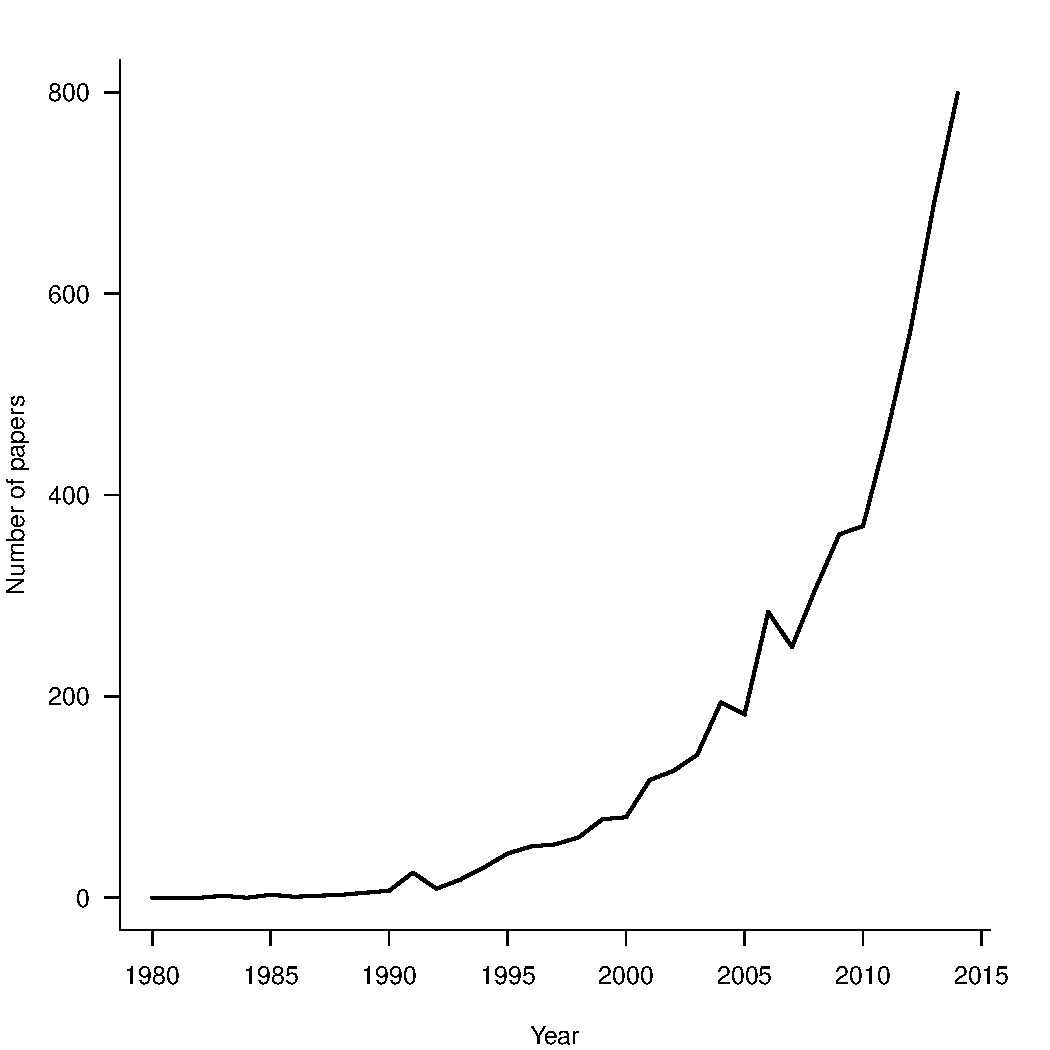
\includegraphics[width=12cm]{Figures/PCMCitations.pdf}
      \caption{The number of papers containing the phrase ``phylogenetic comparative'' published each year from 1980-2014 (Google Scholar search April 13th 2015).}
      \label{PCMCitations}
  \end{figure}

\newpage
  \begin{figure}[!htbp]
    \centering
      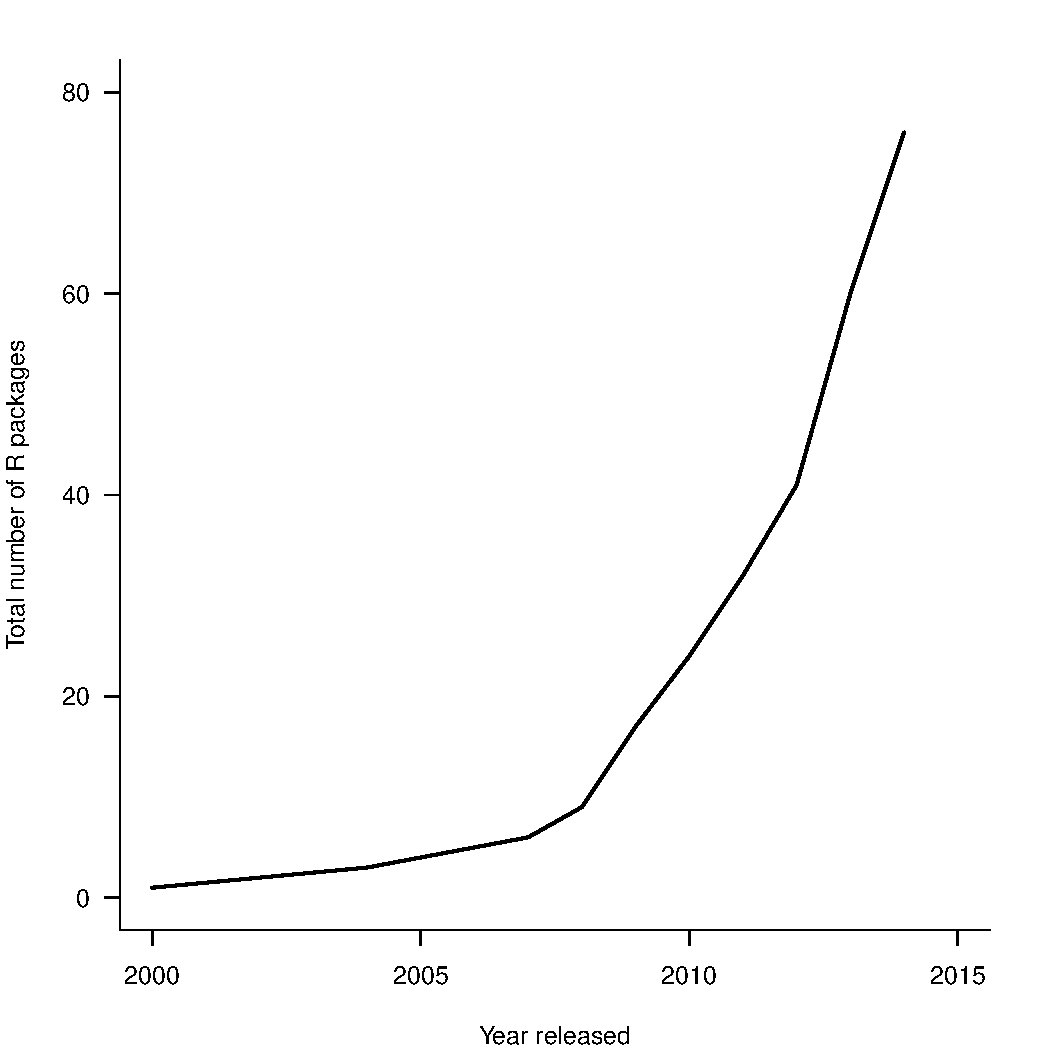
\includegraphics[width=12cm]{Figures/PCMRpackages.pdf}
      \caption{The cumulative total number of R packages for phylogenetics and phylogenetic comparative methods through time from 1980-2014. Source: Brian O'Meara's ``CRAN Task View: Phylogenetics, Especially Comparative Methods'' version 2015-01-21.}
      \label{PCMRpackages}
  \end{figure}

\end{document}
